\newpage
\chapter{Software architecture}\SecLabel{SoftwareArchitecture}
 

\BornAgain\ is written in \Code{C++}
and uses an object oriented approach to 
achieve modularity, extensibility and transparency.
This leads to the task driven rather than the command driven approach in 
different aspects of the simulation and fitting of GISAS data.
The user defines the sample structure, beam and detector characteristics and
fit parameters using building
blocks -- \Code{classes} -- defined in core libraries of the framework.
These buildings blocks are combined by the user according to his current
task using one the following approaches:
\begin{itemize}
\item The user creates a \Python\ script with a sample description and simulation settings
using the \BornAgain\ API.
The user then runs the simulation by executing the script in the \Python\ interpreter and assesses the
simulation results using his preferred graphics or analysis library, e.g. \Python\ + \Code{numpy} + \Code{matplotlib}.
\item The user may write a standalone \Code{C++} application linked to the \BornAgain\ libraries.
\item The user interacts with the framework through a graphical 
user interface (forthcoming).
\end{itemize}

The object oriented approach in the software design allows users 
to have a much higher level of flexibility in the sample construction; it also
decouples the building blocks used in the internal calculations and thereby facilitates the creation of new models,
with little or no modification to the existing code. 


\begin{figure}[htbp]
\centering
  \resizebox{0.9\textwidth}{!}{%
    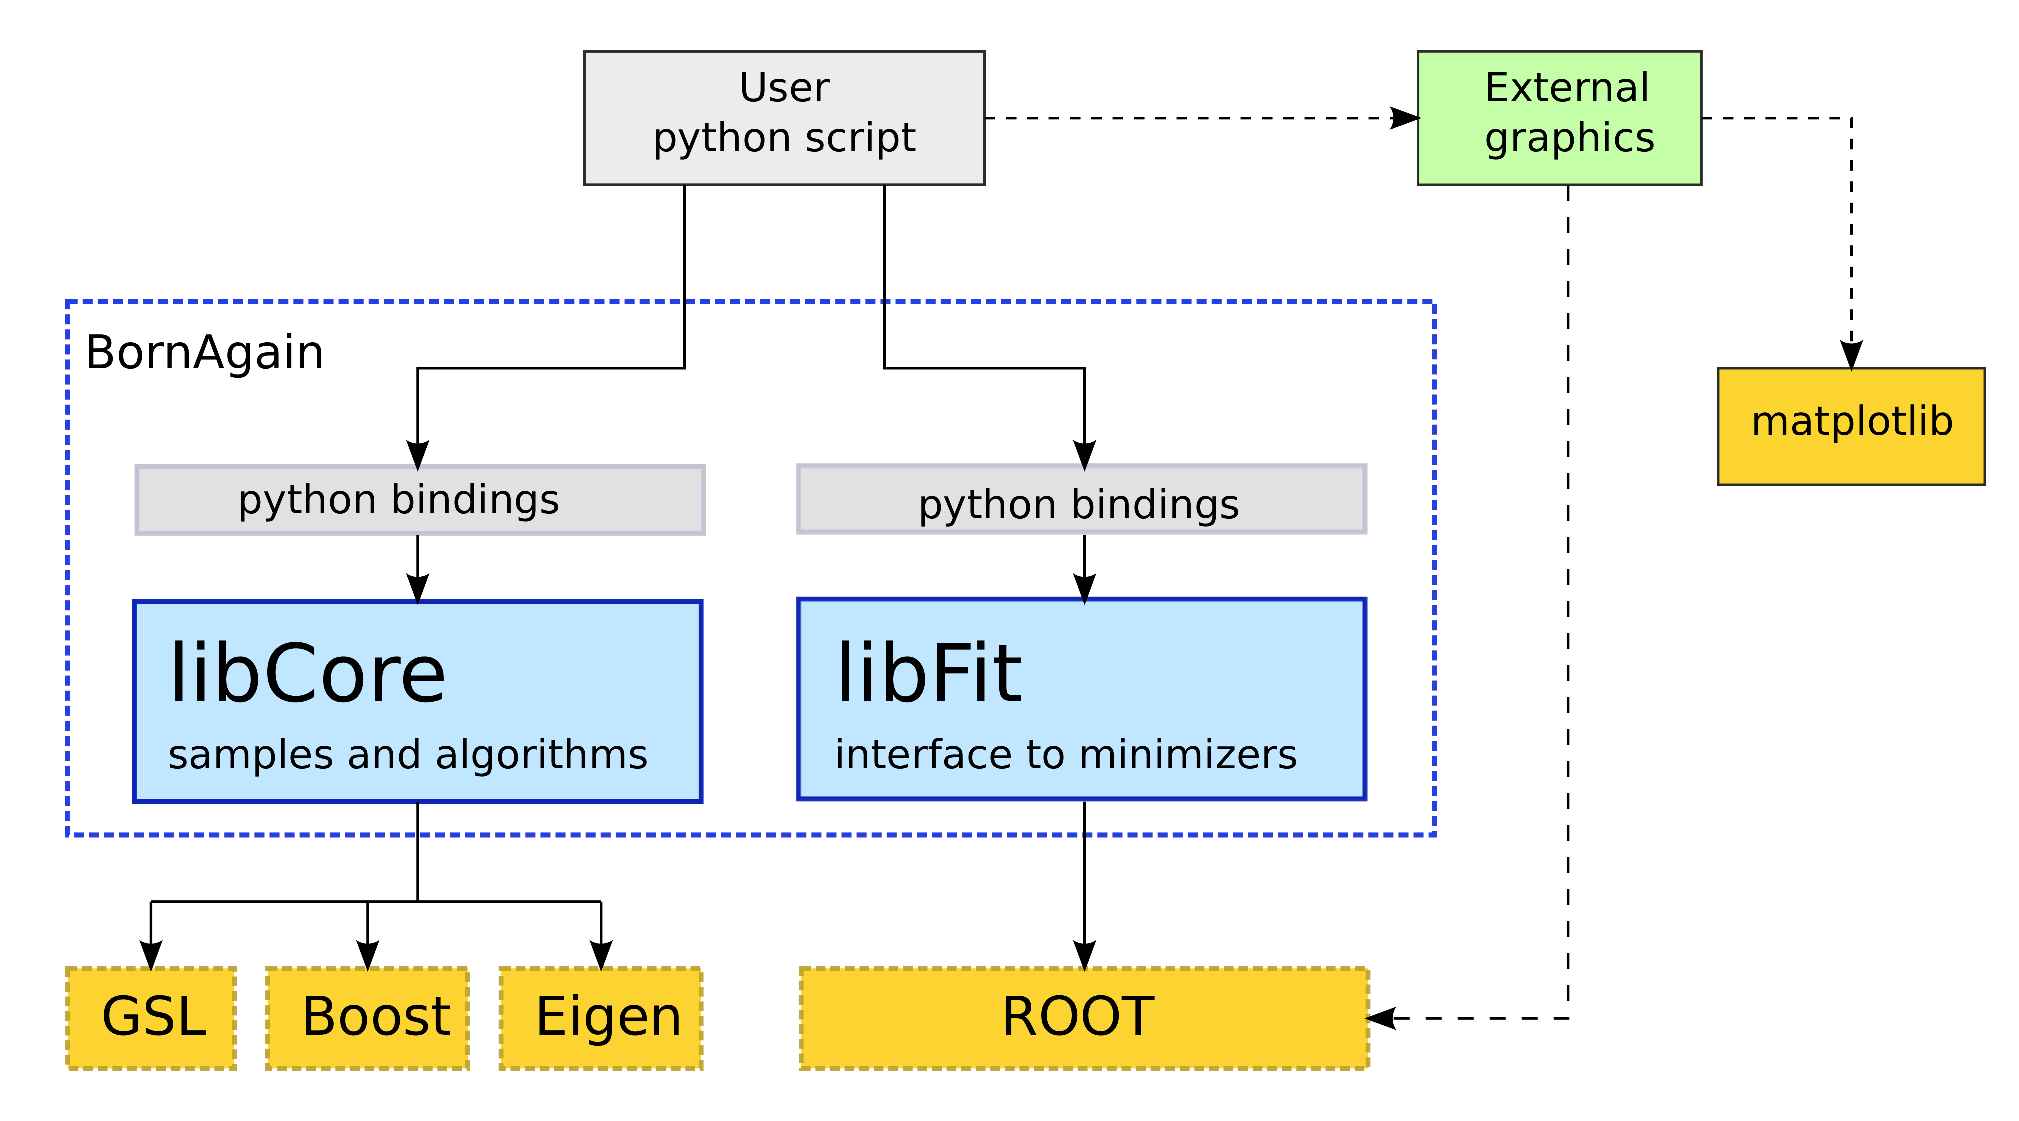
\includegraphics{Figures/basic_architecture.eps}}
\caption{
Structure of \BornAgain\ libraries.
}
\label{fig:two_ratios}
\end{figure}


The general structure of \BornAgain\ and the way the user interacts with it are
shown in Fig.~\ref{fig:two_ratios}.
The framework consists of two shared libraries, \Code{libBornAgainCore} and
\Code{libBornAgainFit}. Thanks to the \Python\ interface they can be imported into \Python\ as external modules. The library \Code{libBornAgainCore} contains a number of classes, grouped into several class categories, necessary for the description of a model and running a simulation.
The library  \Code{libBornAgainFit} contains a number of minimization engines 
and interfaces to them, allowing the user to fit real data with the model previously defined.

\BornAgain\ depends on a few external and well established
open-source libraries: \Code{boost}, GNU scientific library, Eigen and
Fast Fourier Transformation libraries. They are required to be
installed on the system to run \BornAgain\ on Unix Platforms. In the
case of Windows Platform they are added to the system automatically during \BornAgain\ installation. Other libraries shown
on the plot (\Code{ROOT}, \Code{matplotlib}) are optional.

 


%\section{Design overview}

% general considerations
% general capabilities and properties
% openess 
% global structure
% design and architecture

% Software process
% - configuration and release management
% - quality assurance and testing
% - user support process


% The BornAgain framework provides a number of classes, grouped into several class categories.

